\section{Command Line Interface}

The last not yet described part of the GIMMIX simulator is the command line interface. As already mentioned, GIMMIX has the goal to provide a convenient, intuitive and productive interface, to allow it to debug an operating system. Of course, the user needs some commands to work with the simulator, such as "execute one instruction", "print a part of the state" or "disassemble instructions". Additionally, it has been decided to develop a small language, that is used by all commands. The language allows it to access the different entities of MMIX (registers, virtual memory, \dots) and do calculations with them. This way, the user has a lot of flexibility when examining a program, all commands work in a common way and it is easy to add new commands.

\subsection{The Language}

The language is designed to be both usable interactively and non-interactively. That is, when controlling the simulator with the command line interface, it is used interactively. But it is also possible to execute scripts before entering the CLI; for example to establish an initial environment for convenience or to start and control the simulator fully automatized. To achieve that goal, the language consists of an arbitrary number of commands with one command per line. Each line looks like:
\begin{verbatim}
commandName [<arg1> <arg2> ...]
\end{verbatim}
That is, the command name comes first, followed by an arbitrary number of arguments. The command name and the arguments are separated by whitespace. Thus, no whitespace can be used inside an argument. This has been chosen, because it is no general purpose programming language, in which complex expressions are used, but it is intended as a language to use the simulator. That means, it is expected that the user does not want to type more than necessary and whitespace in an expression is not required. Additionally, since it is more a shell language than a programming language, the similarity to popular shell languages has been favored.

Each argument is an expression, whose grammar looks like the following:
\begin{lstlisting}[caption=Grammar of expressions in \protect\gls{EBNF}]
expr = string | integer	| float
	| expr,"+",expr | expr,"-",expr
	| expr,"*",expr | expr,"/",expr | expr,"%",expr
	| expr,"s*",expr | expr,"s/",expr | expr,"s%",expr
	| expr,"&",expr | expr,"|",expr | expr,"^",expr
	| expr,"<<",expr | expr,">>",expr | expr,">>>",expr
	| "~",expr | "-",expr
	| "@"
	| expr,"..",expr | expr,":",expr
	| "M","[",expr,"]"
	| "M1","[",expr,"]" | "M2","[",expr,"]"
	| "M4","[",expr,"]" | "M8","[",expr,"]"
	| "m","[",expr,"]"
	| "l","[",expr,"]" | "g","[",expr,"]"
	| "sp","[",expr,"]"
	| "$","[",expr,"]" | "$",integer
	| "(",expr,")";
\end{lstlisting}
The nonterminal `string` begins with a letter (`[A-Za-z]`), followed by an arbitrary number of alphanumeric characters. An `integer` can be specified in base 2 using the prefix `0b`, octal using `0`, hexadecimal using `0x` or `#` and decimal without a prefix. Additionally, the special registers \sr{A}, \dots, \sr{Z}, \sr{BB}, \sr{SS}, \sr{TT}, \sr{WW}, \sr{XX}, \sr{YY} and \sr{ZZ} are translated into their internal number, so that they can be used at arbitrary places (\eg `sp[rA]`). And a `float` can be specified in the form accepted by the function `strtod` from the C standard library. That means, either by optionally starting with the decimal part, followed by a dot and the fraction part or by using the scientific notation. Thus, for example `1.0`, `.6`, `2.5e1` or `12E-1`.

As the grammar shows, the notation is very similar to the one generally used in this thesis. Additionally, one can see that three data types exist in the language: integers, floating point numbers and strings. Furthermore, it has the following groups of operators:
\begin{itemize}
	\item Arithmetic:\\
	One can use the well known arithmetic operations addition, substraction, multiplication, division and modulo with `+`, `-`, `*`, `/` and `%`, respectively. Additionally, their signed counterpart is available for `*`, `/` and `%` by prefixing it with an "s".
	\item Bit and shift operators:\\
	The bit operations `AND`, `OR` and `XOR` are denoted by `&`, `|` and `^`. Additionally `<<` performs a left shift, `>>` an arithmetic right shift and `>>>` a logical right shift.
	\item Negation:\\
	All values can be negated arithmetically by using `-` and all integers can additionally be negated logically via `~`.
	\item \glslink{PC}{Instruction Pointer}:\\
	The \glslink{PC}{instruction pointer} can be accessed by `@`.
	\item Ranges:\\
	One of the most important and interesting concepts of the language are the so called \i{ranges}. The range `X..Y` corresponds to `X`, `X+1`, \dots, `Y` and the range `X:Y` corresponds to `X`, `X+1`, \dots, `X+Y-1`. Thus, the first one specifies the beginning and end, whereas the second one specifies the beginning and the length.
	\item Fetches:\\
	The last group of operations are the so called \i{fetches}. Analogous to the notation used throughout this thesis, `M` accesses virtual memory, while `m` accesses physical memory. More precisely, `M[x]` denotes the 8 unaligned bytes at location `x`, `M1[x]` denotes the byte at location `x`, `M2[x]` denotes the wyde at wyde-aligned location `x`, `M4[x]` denotes the tetra at tetra-aligned location `x` and finally, `M8[x]` denotes the octa at octa-aligned location `x`. The value of the expression `m[x]` is the octa at octa-aligned physical memory location `x`. Additionally, one can access a local, global and special register `x` via `l[x]`, `g[x]` and `sp[x]`, respectively. Finally, dynamic register `x` can be specified by either `$[x]` or `$x`.
\end{itemize}
It should be noted, that all operations behave like defined in MMIX. That is, unsigned division behaves like \mi{DIVU}, signed division like \mi{DIV} and so on.

% TODO mention that ranges can't be nested?

\subsection{Commands}

GIMMIX provides several commands to allow the user of the simulator to inspect or change the current state, debug and control a program. But of course, it is expected that more commands might be added in future. The following gives an overview of the most important commands and their functional principles.

\subsubsection{Print and Set}

\gcmdtbl{p [<fmt>] <expr..>...}{Print expression(s) in format \gcmd{<fmt>}}
\noindent The print command is one of the most important ones, because it allows it to print arbitrary values or entities of GIMMIX. The argument \gcmd{<fmt>} is optional and can be \gcmd{u} for decimal unsigned, \gcmd{d} for decimal signed, \gcmd{o} for octal unsigned, \gcmd{x} for hexadecimal unsigned, \gcmd{lx} for hexadecimal unsigned with 16 digits (default), \gcmd{f} for float or \gcmd{s} for string. For example, "\gcmd{p \dr{1}}" prints the value of dynamic register 1 and "\gcmd{p o 42}" prints the value 42 in octal base. The ".." after \gcmd{expr} indicates that ranges are supported, while the "..." at the end indicates that multiple arguments of it can be given. That is, "\gcmd{p 1..4}" would print the values 1, 2, 3 and 4 and "\gcmd{p 1 2 3 4}" would do that as well. Additionally, besides printing values or entities of GIMMIX, another useful application of this command is to analyse different representations of values. That is, "\gcmd{p x -8}" to see the hexadecimal representation of $-8$, "\gcmd{p x 1.4}" for the hexadecimal integer representation for the float $1.4$, "\gcmd{p f \#3FF<{}<52}" for the float that is represented by \haddro{3FF0}{0000}{0000}{0000} and so on.

\gcmdtbl{set <obj..> <expr..>}{Set \gcmd{<obj>} to \gcmd{<expr>}}
\noindent The set command can be used to change the state, such as a register, a value at a specific memory location or the \glslink{PC}{instruction pointer}. For example, "\gcmd{set \dr{[1..3]} 10..12}" would set \dr{1} to 10, \dr{2} to 11 and \dr{3} to 12.

\subsubsection{Execution of Instructions}

\gcmdtblfour
	{s [<count>]}{Execute one or \gcmd{<count>} instruction(s)}
	{c [<count>]}{Continue one or \gcmd{<count>} time(s)}
	{ou [<count>]}{Step out of current function one or \gcmd{<count>} time(s)}
	{ov [<count>]}{Step over next instruction one or \gcmd{<count>} time(s)}
\noindent To control the running program, the CLI offers the commands \i{step} (s), \i{continue} (c), \i{stepout} (ou) and \i{stepover} (ov), whereas stepout means that GIMMIX continues until the current function is left via \mi{POP}. If the next instruction is not \mi{PUSHJ} or \mi{PUSHGO}, stepover will execute only this instruction. Otherwise it will continue until the called function is left by \mi{POP}. That is, it "steps over" a function call.

\gcmdtbl{d [<addr..>]}{Disassemble instruction(s) at \gcmd{@} or \gcmd{<addr>}}
\noindent The disassemble command interprets either the tetra at the \glslink{PC}{instruction pointer} or the tetra(s) at \gcmd{<addr>} as instructions and prints their name and operands. For example, "\gcmd{d @:16}" would disassemble the next four instructions at the \gls{PC}.

\gcmdtblthree
	{b v <mode> <addr>}{Break if \gcmd{<addr>} (virt.) is accessed for \gcmd{<mode>} (rwx)}
	{b p <mode> <addr>}{Break if \gcmd{<addr>} (phys.) is accessed for \gcmd{<mode>} (rwx)}
	{b e <expr..>}{Break if the value of \gcmd{<expr>} changed}
\noindent Of course, one has to be able to set breakpoints. GIMMIX provides a very general facility to do so. Because the break command \gcmd{b} can be used to stop the CPU as soon as a specific virtual or physical address is accessed for a specific mode. That is, when specifying \gcmd{x} as mode, it stops the CPU as soon as an instruction should be executed at that position; \ie this would be an ordinary breakpoint. But one can also stop the CPU as soon as a specific memory location is read or written. Additionally, the third version of it offers the opportunity to set expression breakpoints. That means, with "\gcmd{b e \dr{1}}" the CPU would stop as soon as the value of \dr{1} has changed and, as the command description indicates, ranges are supported as well.

\gcmdtbl{e [<flags>]}{Print effects of last instruction}
\noindent To be able to see all effects that an instruction caused, the command \gcmd{e} can be used. It optionally takes an argument with flags, which are any combination of \gcmd{s}, \gcmd{d}, \gcmd{c}, \gcmd{v} and \gcmd{f}. By default, only \gcmd{s} is used. The flag \gcmd{s} prints all reads and writes from/to the stack. Flag \gcmd{c} prints fills and write-backs of the caches, \gcmd{d} prints accesses to the devices and \gcmd{v} prints virtual address translations. Finally, \gcmd{f} specifies that effects, that occur during the fetch phase, are printed as well. For example, a typical output of the command could be:
\begin{verbatim}
8000000000001008: E0016000 (SETH   ): rL=2,$1=l[1] = #6000000000000000
\end{verbatim}
That means, the last executed instruction at location \haddro{8000}{0000}{0000}{1008} was \mi{SETH}, which is encoded by \haddrt{E001}{6000}. Behind the name of the instruction, the effects are displayed. In this case, \dr{1}, currently stored in $l[1]$, has been set to \haddro{6000}{0000}{0000}{0000} and \sr{L} has been increased to 2.

\subsubsection{Examining the State}

\gcmdtblfour
	{itc [<addr..>]}{Print all ITC entries or search for \gcmd{<addr>}}
	{dtc [<addr..>]}{Print all DTC entries or search for \gcmd{<addr>}}
	{ic [<addr..>]}{Print all IC entries or search for \gcmd{<addr>}}
	{dc [<addr..>]}{Print all DC entries or search for \gcmd{<addr>}}
\noindent Of course, the user of the machine should also have the opportunity to print the current content of the caches. Therefore, \gcmd{itc} prints the instruction translation cache, \gcmd{dtc} the data translation cache, \gcmd{ic} the instruction cache and \gcmd{dc} the data cache.

\gcmdtbl{dev}{Print the state of the attached devices}
\noindent Especially when developing or porting an operating system, it is very helpful to see the current state of all devices. Thus, GIMMIX offers this instruction, which prints all devices with their memory range, \glslink{Interrupt}{interrupt} mask and the current device register contents.

\gcmdtbl{tr <cmd> [<arg>...]}{Execute the given command after each CPU stop}
\noindent Another important command is the trace command. It can be used to execute an arbitrary command everytime the CPU stops, \ie as soon as a step, continue or similar is finished. The most frequent usage is probably "\gcmd{tr e}" to display the effect of each instruction. But it can also be used to track the values of registers \dr{4}, \dr{5} and \dr{6} via "\gcmd{tr p \dr{[4..6]}}", for example.

\subsection{Implementation}

After the conceptual description of the command line interface, the most important points of its implementation should be explained.

\subsubsection{General Structure}

The following \gls{FMC} diagram shows the interior of the last black box, displayed in the overview diagram at the beginning:
\begin{figure}[H]
	\centering
	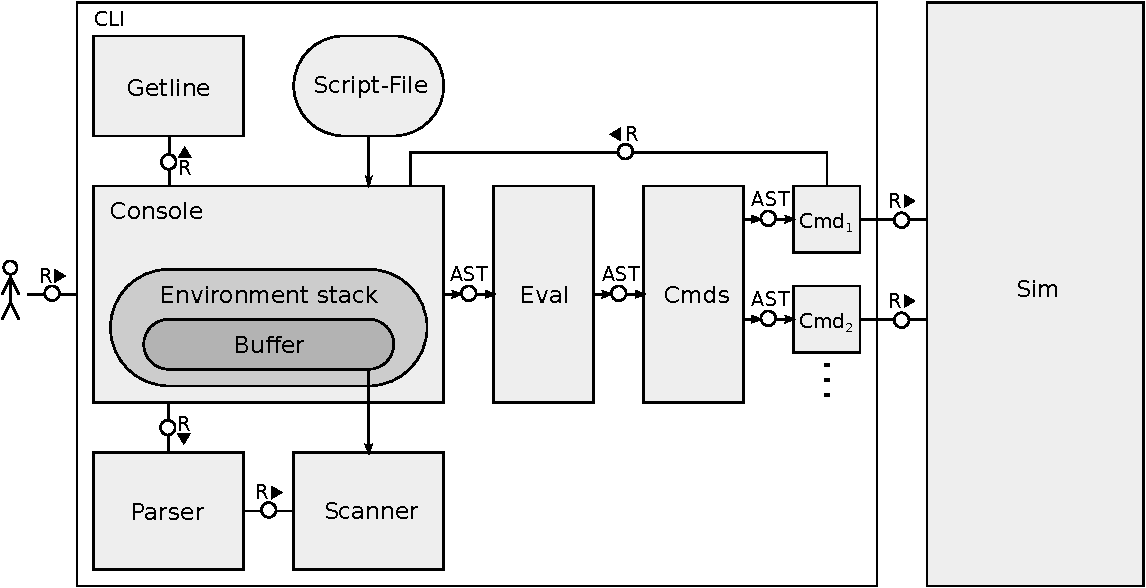
\includegraphics[width=\textwidth]{img/cli-fmc-crop.pdf}
	\caption{Architecture of the CLI in \protect\gls{FMC} notation}
\end{figure}
\noindent Conceptually, the user interacts with the CLI, whose main module is the \i{console}. Depending on whether the console is used interactively or not, it either uses the \i{getline} library\footnote{A small library, that allows basic line editing and provides a history, written by Chris Thewalt. It can be found in the folder \file{lib/getline} of GIMMIX.}  to read a line from the command line into the buffer or reads a specified script file into the buffer. Afterwards this input is parsed to construct an abstract syntax tree (\gls{AST}). The scanner and parser for this task have been generated by \gls{flex} and \gls{Bison}, respectively. As soon as the \gls{AST} is present, it is passed to the \i{eval} module, which executes it. If a node that represents a command is found, the module \i{cmds} comes into play. It holds a table with all available commands and will execute the corresponding function to execute the command. The commands will typically control the simulator, read the state or manipulate it.

As the FMC diagram indicates, the console manages a stack of \i{environments} to allow nesting. Each line or script execution will get a new environment on the top of the stack. This way, a command may use the console to execute a line or script as well. For example, the command \gcmd{tr} uses this feature by storing the desired command as a string and executing it later with the console.

\subsubsection{Command Infrastructure}

Because it is expected that the CLI language itself will not change much in future, but the commands will probably be changed and -- most important -- new ones will be added, it has been decided to separate cleanly between the language and the commands. Additionally, implementing and adding new commands should be as simple as possible. Similarly to the device infrastructure of GIMMIX, a compromise between dynamic and simplicity has been selected. That is, the module cmds keeps a table with all commands, but each command is implemented in its own file. Thus, to add a new command, a file has to be added and the table has to be extended.

Each command has an \i{execution function}, which receives the number of arguments and an array of \gls{AST} nodes -- one for each argument. Additionally, the cmds module provides the function `cmds_evalArg`:
\begin{lstlisting}[language=C]
sCmdArg cmds_evalArg(const sASTNode *arg,int expTypes,octa offset,bool *finished);
\end{lstlisting}
The function receives the argument to evaluate, the types that are supported (integer, float or string), an offset and a pointer to a boolean. The last two are used to implement ranges. Since the language is intended for scripting as well and it is imaginable that a user would like to, \eg, execute 1000 instructions and pipe the contents of the first 64 megabytes of memory into a file to analyze it with other tools later, it has been decided not to simply convert a range to an array. Because as the example shows, it might cost a lot of time and memory. Instead, the evaluation function receives the current offset and tells the caller whether all ranges are already finished. That means, in each step one value of each range is extracted, depending on the current offset.

The return value of `cmds_evalArg` is a struct called `sCmdArg`, that provides all required information about the value of the argument for the caller. It contains the type (integer, float or string), the origin (\gcmd{M8}, \gcmd{l}, \gcmd{\$}, and so on or an arbitrary expression such as \gcmd{1+2}), the location for origins like virtual memory or registers (that is, the memory address or register index) and of course the value of the argument as integer, float or string. The location and origin are for example used by \gcmd{p} to print the origin of an argument or by \gcmd{set} to set the corresponding entity of GIMMIX.

\subsubsection{Command Implementation}

A typical command, that makes use of ranges, is \i{disassemble}. Ignoring the details of the disassembling process, its implementation looks like the following:
\begin{lstlisting}[language=C,caption={Implementation of command \gcmd{d}}]
void cli_cmd_disasm(size_t argc,const sASTNode **argv) {
	if(argc > 1)
		cmds_throwEx(NULL);
	if(argc == 0)
		doDisasm(cpu_getPC());
	else {
		sCmdArg a;
		bool fin = false;
		for(octa off = 0; ; off += sizeof(tetra)) {
			a = cmds_evalArg(argv[0],ARGVAL_INT,off,&fin);
			if(fin)
				break;
			doDisasm(a.d.integer & -(octa)(sizeof(tetra));
		}
	}
}
\end{lstlisting}
As the listing shows, at first the number of arguments is checked and if no arguments are given, one instruction at the PC will be disassembled. If one argument is given, `cmds_evalArg` will be called until `fin` has been set to `true`, whereas in each step the offset `off` will be increased to reach the next instruction. Thus, "\gcmd{d @:16}" would disassemble the instructions at addresses `@`, `@+4`, `@+8` and `@+12`.

Another interesting example, that utilizes the origin and location, is the command \gcmd{set}. The slightly shortened implementation is:
\begin{lstlisting}[language=C,caption={Implementation of command \gcmd{set}}]
void cli_cmd_set(size_t argc,const sASTNode **argv) {
	if(argc != 2)
		cmds_throwEx(NULL);
	for(octa off = 0; ; off++) {
		bool oFin = false, vFin = false;
		sCmdArg obj,val;
		obj = cmds_evalArg(argv[0],ARGVAL_INT,off,&oFin);
		val = cmds_evalArg(argv[1],
			ARGVAL_INT | ARGVAL_FLOAT,off,&vFin);
		if(oFin)
			break;

		switch(obj.origin) {
			case ORG_VMEM1:
				mmu_writeByte(obj.location,val.d.integer,0);
				break;
			...
			case ORG_EXPR:
				cmds_throwEx("Can't set arbitrary expr\n");
				break;
		}
	}
}
\end{lstlisting}
That means, it iterates over both the objects to set and the values at the same time, until the last object has been assigned. Additionally, the origin is used to determine what entity of GIMMIX should be changed. Of course, \gcmd{set} is not possible for expressions like \gcmd{1*2+M[0]} as first argument. It is only allowed for the \glslink{PC}{instruction pointer} and for fetches, that are specified without any operator in the "outmost layer", \ie \gcmd{M4[@+4]} for example.

